\documentclass[conference]{IEEEtran}
\IEEEoverridecommandlockouts
% The preceding line is only needed to identify funding in the first footnote. If that is unneeded, please comment it out.
\usepackage{cite}
\usepackage{amsmath,amssymb,amsfonts}
\usepackage{algorithmic}
\usepackage{graphicx}
\usepackage{textcomp}
\usepackage{xcolor}
\def\BibTeX{{\rm B\kern-.05em{\sc i\kern-.025em b}\kern-.08em
    T\kern-.1667em\lower.7ex\hbox{E}\kern-.125emX}}
\begin{document}

\title{Prediction of Covid-19  according to different symptoms}

\author{\IEEEauthorblockN{Sarder Iftekhar Ahmed}
\IEEEauthorblockA{\textit{2018-1-60-181} \\
\textit{East West University}\\
email:2018-1-60-181@std.ewubd.edu}
\and
\IEEEauthorblockN{Md. Nadim}
\IEEEauthorblockA{\textit{2018-1-60-161} \\
\textit{East West University}\\
email:2018-1-60-161@std.ewubd.edu}
\and
\IEEEauthorblockN{Md Mizanur Rahman}
\IEEEauthorblockA{\textit{2018-1-60-249} \\
\textit{East West University}\\
email:2018-1-60-249@std.ewubd.edu}
}
\maketitle

\begin{abstract}
 Covid-19 has been a global concern for more than a year and a half. Covid-19 is an infectious disease that is very important to diagnose, but the detection kit is expensive. And because it is time consuming, people are avoiding testing, which is contributing to the spread of infection .Technology advancements have a rapid effect on every field of life; it can be medical field or any other field. Artificial intelligence has shown us better development in health sector by its own decision making and analyzing the data. At this time, our world are going through global pandemic situations. Corona virus has affected most of the country in the world. People have nothing to do except suffering and going through this matter. So, Developing a control system that will detect corona virus will be lifesaving at this moment.  we have developed such a tool that will predict covid-19. For making this happen, we used naïve Bayes and a data sheet that we find on internet.

\end{abstract}

\begin{IEEEkeywords}
Corona Virus, Naïve Bayes, Machine learning.
\end{IEEEkeywords}

\section{Introduction}
The novel coronavirus emerged in Wuhan city of China in December 2019 and was informed to the World Health Organization (W.H.O) on 31st December 2019. The virus formed a global threat and was named as COVID-19 by W.H.O on 11th February 2020. The COVID-19 comes from the family of viruses including SARS, ARDS. W.H.O declared this outbureak as a public health emergency and stated the following; the virus is being transmitted via the respiratory tract when a healthy person comes in contact with the infected person. The virus may spread between persons through other roots which are currently uncertain. The infected person shows symptoms within 2–14 days, depending on the incubation period of the middle east respiratory syndrome (MERS), and the severe acute respiratory syndrome (SARS). According to WHO the signs and indications of mild to moderate cases are dry cough, fatigue and fever while as in severe cases dyspnea (shortness of breath), Fever and tiredness may transpire. The persons having other diseases like asthma, diabetes, and heart disease are more exposed to  the virus and maybecome severely ill. The person is diagnoses based on symptoms and his travel history. Vital signs are being experimental keenly of the client having symptoms. By washing hands regularly with soap for at least 20 seconds and avoiding close body contact with others by keeping the distance of about 3 meter may reduce the chances of getting affected by this virus. While sneezing, covering the mouth and nose with the help of throwaway tissue and avoiding the contact with the nose, ear and mouth can help in its prevention. Till 23th of May 2021, almost 167 million confirmed cases of coronavirus are spotted around the globe. Almost 3.4 million persons have died and 148 million persons have recovered from this deadly virus. Figure 1 displays the worldwide data regarding coronavirus. Less time and man- power in testing have also given rise to this disease as we lack the medical resources due to pandemic. Since thousands of people are being tested positive every day around the globe, it is not possible to test all these people who show symptoms Apart from clinical procedures, machine learning provides a lot of support in detecting the disease with the help of image and textual data. Machine learning can be used for the identification of novel coronavirus. It can also predict the nature of the virus across the globe. However, machine learning requires a large amount of data for classifying or foreseeing diseases. Supervised machine learning algorithms need marked data for classifying the text or image into different categories. From the past decade, a large amount of growth is being made in this area for resolving some critical projects. Recent pandemic has attracted many researchers around the globe to resolve this problem. So, this is no surprise that covid-19 is a big concern for us , people are implementing many approaches and doing many research to prevent and detecting corona virus. In this project, we will discuss about the detection of corona virus based on different symptoms using Naïve Bayes classifier.
\section{Related Work}
Machine learning and natural language processing uses big data-based replicas for pattern recognition, explanation, and prediction. NLP has expanded much interest in recent years, mostly in the field of text analytics, Classification is one of the foremost tasks in text mining and can be accomplished using different algorithms. Kumar et al performed a SWOT analysis of various supervised and unsupervised text classification algorithms for mining the unstructured data\cite{kumar2020text}. The various applications of text classification are sentiment analysis, fraud detection, and spam detection etc. Opinion mining is majorly being cast-off for elections, advertisement, business etc. Verma et al analyzed Sentiments of Indian government projects with the help of the lexicon-based dictionary\cite{verma2019twitter}. The machine learning has changed the viewpoint of diagnosis by giving great results to diseases like diabetes and epilepsy. These purposes can be helpful to diagnose and predict COVID-19. Firm and exact diagnosis of COVID-19 can save millions of lives and can harvest a massive amount of data on which a machine learning (ML) models can be trained. ML may provide useful input in this favor, in particular in making diagnoses based on clinical text, radiography Images etc. According to Bullock et al, Machine learning and deep learning can substitute humans by giving an accurate diagnosis. The perfect diagnosis can save radiologists’ time and can be cost-effective than normal tests for COVID-
19\cite{bullock2020mapping}. X-rays and computed tomography (CT) scans can be used for training the machine learning model. Several initiatives are ongoing in this regard. Wang and Wong developed COVID-Net, which is a deep convolutional neural network, which can diagnose COVID-19 from chest radiography images\cite{wang2020covid}. Once the COVID-19 is detected in a person, the query is whether and how intensively that person will be affected. Not all COVID-19 positive patients will need rigorous consideration. Being able to prognosis who will be affected more severely can help in directing assistance and planning medical resource allocation and application. Jiang et al proposed a machine learning model that can foresee a person affected with COVID-19 and has the possibility to develop   acute   respiratory distress syndrome
 
(ARDS)\cite{xu2021risk}. The projected model resulted in 80\% of accuracy. The samples of 53 patients were used for training their model and are limited to two Chinese hospitals. Since less work is being done on detecting corona virus, we used machine learning Naïve Bayes algorithm to detect corona virus based on different symptoms.



\section{Methodology}

Our proposed project methodology consists of two different steps one is data collection and another one is machine-learning classification. In the given diagram below, we try to show our entire methodology. At machine learning classification, we will discuss about which machine-learning algorithm we are going to use for this proposal project.


\begin{figure}[h!]
    \centering
    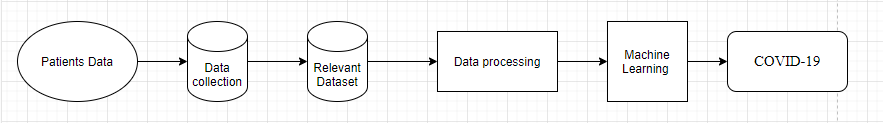
\includegraphics[scale=0.2]{flow.png}
    \caption{Control Flow Diagram}
    \label{fig:flow}
\end{figure}



\subsection{Data Collection}
As the World Health Organization declared health emergency because of Corona virus pandemic
 
around the globe. All the researcher and hospitals around the world has given open access to the data about this digester. As a result, we managed to collect our data from open-source data repository on the internet. In which, 1001 rows of data is sorted which have shown symptoms and results of corona virus affected peoples. Data consists of about different attributes such as serial number, Gender, Temperature, cough, Tiredness difficulty, Loss of taste, Sore throat and result of covid-19.


\subsection{Machine-Learning Classsification}
In this project, we used Naïve Bayes classifier for corona virus results prediction. A Naïve Thomas Bayes classifier could be a supervised machine- learning formula that utilize Bayes Theorem. In which, we predict that feature are statically non- depended. It actually depends on the Naïve prediction that input variable are freelance of every alternative. There is no thanks to acknowledge something concerning alternative variable once given a further variable. In any case of this prediction, it has justified itself to be a classifier with good results.
Naïve Bayes classifier depends on the Bayes Theorem, which is based on conditional probability, the likelihood that an event will occur given that another event has already took place. Basically, this Theorem help a hypothesis to be modified all the time as new evidence is introduced, the equation give below expresses Bayes theorem within the language of probability.


Bayes theorem gives a way of calculating posterior probability P (A|B) from P(A), P(B) and P (B|A). Look at the equation \ref{fig:like}



 \begin{figure}[h!]
    \centering
    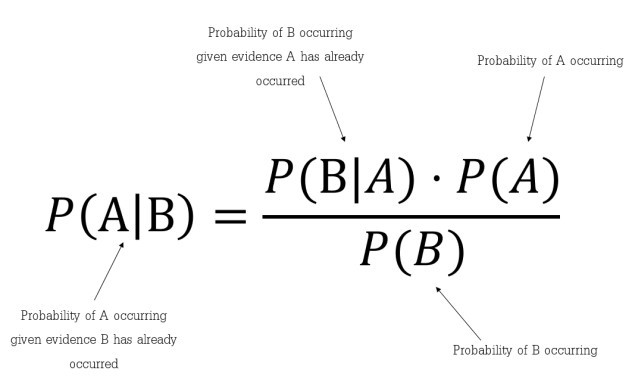
\includegraphics[scale=0.4]{like.jpg}
    \caption{}
    \label{fig:like}
\end{figure}



Bayes theorem above,


P (A|B) is the posterior probability of class (A, target) given predictor (B, attributes).
P(A) is the prior probability of class.

P (B|A) is the likelihood, which is the probability of predictor given class.
P(B) is the prior probability of predictor.

Let us understand it using our example; below we have a data of covid-19 results based on different symptoms. Now, we need to classify whether people are covid-19 affected or not based on the data of the table.

\begin{figure}[h!]
    \centering
    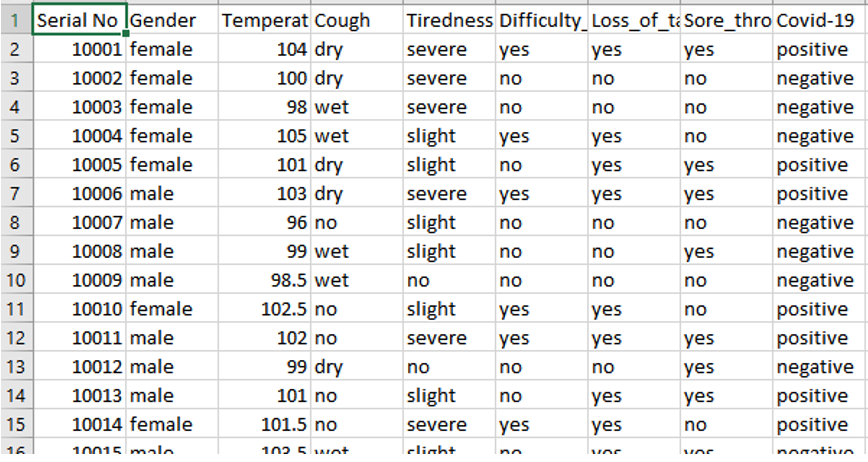
\includegraphics[scale=0.5]{data.PNG}
    \caption{data Set}
    \label{fig:data}
\end{figure}


Step-1: convert the data into a frequency table.
 
Step-2: create likelihood data table by finding the probabilities like overcast probability.
Step-3: At last, we use Naïve Bayes equation to calculate the posterior probability for each class. The class with the most superior posterior probability is the outcome of the prediction.




\section{Results & Discussion}

we used a windows system with 12 GB Ram and 3.4 GHz processor for performing this work. Jupiter notebook tools used for running our machine learning algorithm with the help of different libraries for improving our results.
\subsection{Preprocessing}
The dataset had to be processed in several ways. First, we have to find the unique attribute and total value of deciding factor to find the number of positive and negative people. Then, we find the probabilities of both positive and negative people affected people from data sheet.



\subsection{Testing And Evaluation}
As we said before, we have used Naïve Bayes classifier in this project and our results pretty much as our expectations. We have shown a sample of our results below this.

\begin{figure}[h!]
    \centering
    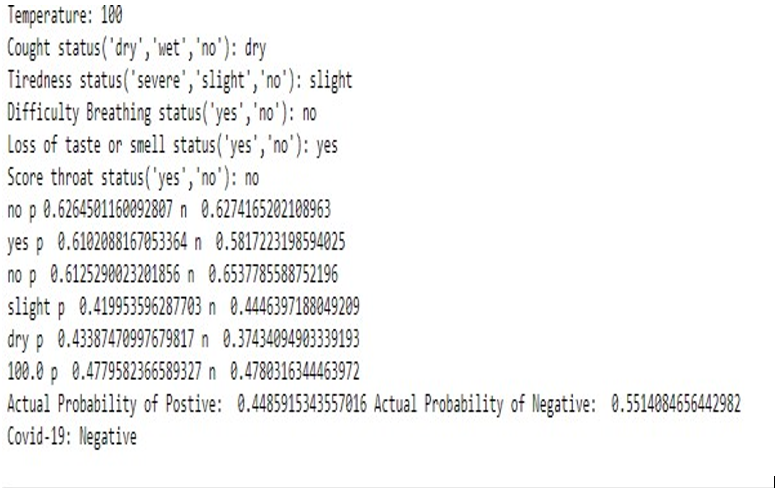
\includegraphics[scale=0.5]{result.PNG}
    \caption{result}
    \label{fig:res}
\end{figure}



\section{Conclusion}
 We used 1001 rows data reports, which are characterized in different classes. The machine learning algorithms are used for finding the probabilities of covid-19. After performing classification, it was discovered that Naïve Bayesian classifier gives excellent results. Various other machine learning algorithms that displayed better results were random forest, stochastic gradient boosting, decision trees and boosting. The efficiency of models can be enhanced by increasing the amount of data. Also, the disease can be classified on the gender-based such that we can get info about whether the males are affected more or females. More featured engineering is needed for better results and deep learning approach can be used in future.


\bibliographystyle{ieeetr}
\bibliography{reference}

\end{document}
